\documentclass[openany]{book}
\usepackage{lmodern}
\usepackage{amssymb,amsmath}
\usepackage{ifxetex,ifluatex}
\usepackage{fixltx2e} % provides \textsubscript
\ifnum 0\ifxetex 1\fi\ifluatex 1\fi=0 % if pdftex
  \usepackage[T1]{fontenc}
  \usepackage[utf8]{inputenc}
\else % if luatex or xelatex
  \ifxetex
    \usepackage{mathspec}
  \else
    \usepackage{fontspec}
  \fi
  \defaultfontfeatures{Ligatures=TeX,Scale=MatchLowercase}
\fi
% use upquote if available, for straight quotes in verbatim environments
\IfFileExists{upquote.sty}{\usepackage{upquote}}{}
% use microtype if available
\IfFileExists{microtype.sty}{%
\usepackage{microtype}
\UseMicrotypeSet[protrusion]{basicmath} % disable protrusion for tt fonts
}{}
\usepackage[margin=1in]{geometry}
\usepackage{hyperref}
\hypersetup{unicode=true,
            pdftitle={DATA 624: Project 1},
            pdfauthor={Juliann McEachern},
            pdfborder={0 0 0},
            breaklinks=true}
\urlstyle{same}  % don't use monospace font for urls
\usepackage{natbib}
\bibliographystyle{plainnat}
\usepackage{color}
\usepackage{fancyvrb}
\newcommand{\VerbBar}{|}
\newcommand{\VERB}{\Verb[commandchars=\\\{\}]}
\DefineVerbatimEnvironment{Highlighting}{Verbatim}{commandchars=\\\{\}}
% Add ',fontsize=\small' for more characters per line
\usepackage{framed}
\definecolor{shadecolor}{RGB}{248,248,248}
\newenvironment{Shaded}{\begin{snugshade}}{\end{snugshade}}
\newcommand{\AlertTok}[1]{\textcolor[rgb]{0.94,0.16,0.16}{#1}}
\newcommand{\AnnotationTok}[1]{\textcolor[rgb]{0.56,0.35,0.01}{\textbf{\textit{#1}}}}
\newcommand{\AttributeTok}[1]{\textcolor[rgb]{0.77,0.63,0.00}{#1}}
\newcommand{\BaseNTok}[1]{\textcolor[rgb]{0.00,0.00,0.81}{#1}}
\newcommand{\BuiltInTok}[1]{#1}
\newcommand{\CharTok}[1]{\textcolor[rgb]{0.31,0.60,0.02}{#1}}
\newcommand{\CommentTok}[1]{\textcolor[rgb]{0.56,0.35,0.01}{\textit{#1}}}
\newcommand{\CommentVarTok}[1]{\textcolor[rgb]{0.56,0.35,0.01}{\textbf{\textit{#1}}}}
\newcommand{\ConstantTok}[1]{\textcolor[rgb]{0.00,0.00,0.00}{#1}}
\newcommand{\ControlFlowTok}[1]{\textcolor[rgb]{0.13,0.29,0.53}{\textbf{#1}}}
\newcommand{\DataTypeTok}[1]{\textcolor[rgb]{0.13,0.29,0.53}{#1}}
\newcommand{\DecValTok}[1]{\textcolor[rgb]{0.00,0.00,0.81}{#1}}
\newcommand{\DocumentationTok}[1]{\textcolor[rgb]{0.56,0.35,0.01}{\textbf{\textit{#1}}}}
\newcommand{\ErrorTok}[1]{\textcolor[rgb]{0.64,0.00,0.00}{\textbf{#1}}}
\newcommand{\ExtensionTok}[1]{#1}
\newcommand{\FloatTok}[1]{\textcolor[rgb]{0.00,0.00,0.81}{#1}}
\newcommand{\FunctionTok}[1]{\textcolor[rgb]{0.00,0.00,0.00}{#1}}
\newcommand{\ImportTok}[1]{#1}
\newcommand{\InformationTok}[1]{\textcolor[rgb]{0.56,0.35,0.01}{\textbf{\textit{#1}}}}
\newcommand{\KeywordTok}[1]{\textcolor[rgb]{0.13,0.29,0.53}{\textbf{#1}}}
\newcommand{\NormalTok}[1]{#1}
\newcommand{\OperatorTok}[1]{\textcolor[rgb]{0.81,0.36,0.00}{\textbf{#1}}}
\newcommand{\OtherTok}[1]{\textcolor[rgb]{0.56,0.35,0.01}{#1}}
\newcommand{\PreprocessorTok}[1]{\textcolor[rgb]{0.56,0.35,0.01}{\textit{#1}}}
\newcommand{\RegionMarkerTok}[1]{#1}
\newcommand{\SpecialCharTok}[1]{\textcolor[rgb]{0.00,0.00,0.00}{#1}}
\newcommand{\SpecialStringTok}[1]{\textcolor[rgb]{0.31,0.60,0.02}{#1}}
\newcommand{\StringTok}[1]{\textcolor[rgb]{0.31,0.60,0.02}{#1}}
\newcommand{\VariableTok}[1]{\textcolor[rgb]{0.00,0.00,0.00}{#1}}
\newcommand{\VerbatimStringTok}[1]{\textcolor[rgb]{0.31,0.60,0.02}{#1}}
\newcommand{\WarningTok}[1]{\textcolor[rgb]{0.56,0.35,0.01}{\textbf{\textit{#1}}}}
\usepackage{graphicx,grffile}
\makeatletter
\def\maxwidth{\ifdim\Gin@nat@width>\linewidth\linewidth\else\Gin@nat@width\fi}
\def\maxheight{\ifdim\Gin@nat@height>\textheight\textheight\else\Gin@nat@height\fi}
\makeatother
% Scale images if necessary, so that they will not overflow the page
% margins by default, and it is still possible to overwrite the defaults
% using explicit options in \includegraphics[width, height, ...]{}
\setkeys{Gin}{width=\maxwidth,height=\maxheight,keepaspectratio}
\IfFileExists{parskip.sty}{%
\usepackage{parskip}
}{% else
\setlength{\parindent}{0pt}
\setlength{\parskip}{6pt plus 2pt minus 1pt}
}
\setlength{\emergencystretch}{3em}  % prevent overfull lines
\providecommand{\tightlist}{%
  \setlength{\itemsep}{0pt}\setlength{\parskip}{0pt}}
\setcounter{secnumdepth}{5}

%%% Use protect on footnotes to avoid problems with footnotes in titles
\let\rmarkdownfootnote\footnote%
\def\footnote{\protect\rmarkdownfootnote}

%%% Change title format to be more compact
\usepackage{titling}

% Create subtitle command for use in maketitle
\providecommand{\subtitle}[1]{
  \posttitle{
    \begin{center}\large#1\end{center}
    }
}

\setlength{\droptitle}{-2em}

  \title{DATA 624: Project 1}
    \pretitle{\vspace{\droptitle}\centering\huge}
  \posttitle{\par}
    \author{Juliann McEachern}
    \preauthor{\centering\large\emph}
  \postauthor{\par}
      \predate{\centering\large\emph}
  \postdate{\par}
    \date{October 22, 2019}

\usepackage{booktabs}
\usepackage[table]{xcolor}

% set plain style for page numbers
\pagestyle{plain}
\raggedbottom

% change font
\usepackage{fontspec}
\setmainfont{Arial}

% remove "chapter" from chapter title
\usepackage{titlesec}
\titleformat{\chapter}
  {\normalfont\LARGE\bfseries}{\thechapter}{1em}{}
\titlespacing*{\chapter}{0pt}{3.5ex plus 1ex minus .2ex}{2.3ex plus .2ex}

% create color block quotes
\usepackage{tcolorbox}
\newtcolorbox{myquote}{colback=orange!05!white, colframe=black!75!black}
\renewenvironment{quote}{\begin{myquote}}{\end{myquote}}

% wrap text
\usepackage{geometry}[textwidth=6in]

% kable 
\usepackage{tabu}
\usepackage{float}
\usepackage{booktabs}
\usepackage{longtable}
\usepackage{array}
\usepackage{multirow}
\usepackage{wrapfig}
\usepackage{float}
\usepackage{colortbl}
\usepackage{pdflscape}
\usepackage{tabu}
\usepackage{threeparttable}
\usepackage{threeparttablex}
\usepackage[normalem]{ulem}
\usepackage{makecell}
\usepackage{xcolor}

\begin{document}
\maketitle

{
\setcounter{tocdepth}{1}
\tableofcontents
}
\hypertarget{overview}{%
\chapter*{Overview}\label{overview}}
\addcontentsline{toc}{chapter}{Overview}

\begin{quote}
I am leaving the project overview page here for us to compile our final
report in one singular document. We will add additional information here
regarding project one to include explanation of process, etc.
\end{quote}

\hypertarget{dependencies}{%
\section*{Dependencies}\label{dependencies}}
\addcontentsline{toc}{section}{Dependencies}

\begin{quote}
Please add all libraries used here.
\end{quote}

The following R libraries were used to complete Project 1:

\begin{Shaded}
\begin{Highlighting}[]
\CommentTok{# General}
\KeywordTok{library}\NormalTok{(}\StringTok{'easypackages'}\NormalTok{)}

\KeywordTok{libraries}\NormalTok{(}\StringTok{'knitr'}\NormalTok{, }\StringTok{'kableExtra'}\NormalTok{, }\StringTok{'default'}\NormalTok{)}

\CommentTok{# Processing}
\KeywordTok{libraries}\NormalTok{(}\StringTok{'readxl'}\NormalTok{, }\StringTok{'tidyverse'}\NormalTok{, }\StringTok{'janitor'}\NormalTok{, }\StringTok{'lubridate'}\NormalTok{)}

\CommentTok{# Graphing}
\KeywordTok{libraries}\NormalTok{(}\StringTok{'ggplot2'}\NormalTok{, }\StringTok{'grid'}\NormalTok{, }\StringTok{'gridExtra'}\NormalTok{, }\StringTok{'ggfortify'}\NormalTok{,}\StringTok{'ggpubr'}\NormalTok{)}

\CommentTok{# Timeseries }
\KeywordTok{libraries}\NormalTok{(}\StringTok{'urca'}\NormalTok{, }\StringTok{'tseries'}\NormalTok{, }\StringTok{'timetk'}\NormalTok{)}

\CommentTok{# Math}
\KeywordTok{libraries}\NormalTok{(}\StringTok{'forecast'}\NormalTok{)}
\end{Highlighting}
\end{Shaded}

\hypertarget{data}{%
\section*{Data}\label{data}}
\addcontentsline{toc}{section}{Data}

Data was stored within our group repository and imported below using the
\texttt{readxl} package. Each individual question was solved within an R
script and the data was sourced into our main report for discussion
purposes. The R scripts are available within our appendix for
replication purposes. For grading purposes, we exported and saved all
forecasts as a csv in our data folder.

\begin{Shaded}
\begin{Highlighting}[]
\CommentTok{# Data Aquisition}
\NormalTok{atm_data <-}\StringTok{ }\KeywordTok{read_excel}\NormalTok{(}\StringTok{"data/ATM624Data.xlsx"}\NormalTok{) }
\NormalTok{power_data <-}\StringTok{ }\KeywordTok{read_excel}\NormalTok{(}\StringTok{"data/ResidentialCustomerForecastLoad-624.xlsx"}\NormalTok{) }
\NormalTok{pipe1_data <-}\StringTok{ }\KeywordTok{read_excel}\NormalTok{(}\StringTok{"data/Waterflow_Pipe1.xlsx"}\NormalTok{)}
\NormalTok{pipe2_data <-}\StringTok{ }\KeywordTok{read_excel}\NormalTok{(}\StringTok{"data/Waterflow_Pipe2.xlsx"}\NormalTok{)}

\CommentTok{# Source Code}
\KeywordTok{source}\NormalTok{(}\StringTok{"scripts/Part-A-JM.R"}\NormalTok{)}
\end{Highlighting}
\end{Shaded}

\hypertarget{part-a}{%
\chapter{Part A}\label{part-a}}

\begin{quote}
\textbf{Instructions:} In part A, I want you to forecast how much cash
is taken out of 4 different ATM machines for May 2010. The data is given
in a single file. The variable \texttt{Cash} is provided in hundreds of
dollars, other than that it is straight forward. I am being somewhat
ambiguous on purpose. I am giving you data, please provide your written
report on your findings, visuals, discussion and your R code all within
a Word readable document, except the forecast which you will put in an
Excel readable file. I must be able to cut and paste your R code and run
it in R studio. Your report must be professional - most of all -
readable, EASY to follow. Let me know what you are thinking, assumptions
you are making! Your forecast is a simple CSV or Excel file that MATCHES
the format of the data I provide.
\end{quote}

\hypertarget{exploration}{%
\section{Exploration}\label{exploration}}

The data covers a period of Friday May 1, 2010 through Saturday April
30, 2010. While reviewing the data, we identified that the original data
file contained \texttt{NA} values in our \texttt{ATM} and \texttt{Cash}
columns for 14 observations between May 1 and 14, 2010. As these contain
no information, we removed these missing values and transformed the
dataset into a wide format.

Our initial review also revealed that ATM2 contained one missing value
on 2009-10-25 and that ATM4 contained a potential outlier of \$1,123 on
2010-02-09. We replaced both values with the corresponding mean value of
each machine.

We examined summary statistics for each ATM time series:

\begin{itemize}
\tightlist
\item
  ATM1 and ATM2 have pretty normal distributions; ATM1's daily mean cash
  dispensed is \$84, and ATM2's is \$62.
\item
  ATM3 only dispensed cash on the last three days of the time series -
  as this provides few data points on which to forecast, we'll need to
  treat it specially.
\item
  ATM4 has a similar mean to ATM1, but skew and kurtosis suggest the
  impact of an outlier Wednesday, February 10, 2010. If this ATM is
  located in the Northeastern United States, this may have a
  relationship to a blizzard which struck on that day.
\end{itemize}

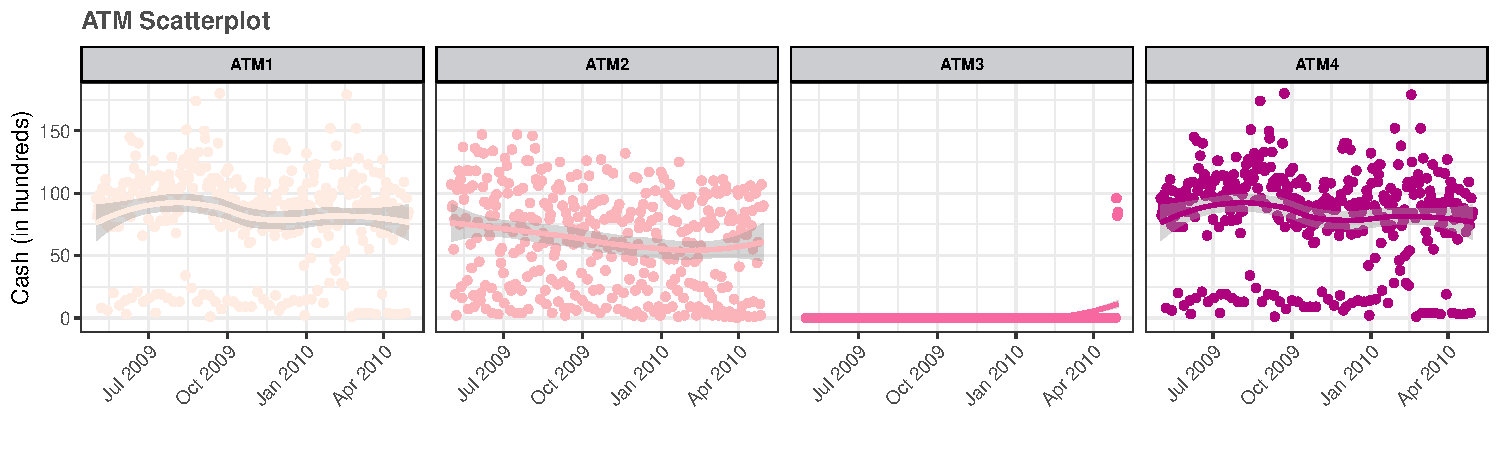
\includegraphics{Part-A-JM_JO_files/figure-latex/unnamed-chunk-3-1.pdf}

Last, we used a scatterplot to examine the correlation between cash
withdrawals and dates for each machine. We identified similiar patterns
between ATM1 and ATM4, which show non-linear fluctuations that suggest a
potential trend component in these timeseries. ATM2 follows a relatively
linear path and decreases overtime. This changes in the last few
observations, where withdrawals begin to increase. As mentioned, there
are only 3 observed transactions for ATM3 that appear at the end of the
captured time period.

\hypertarget{timeseries-plots}{%
\section{Timeseries Plots}\label{timeseries-plots}}

Our cleaned dataframe was then converted into a timeseries format. The
time series plots show high weekly variance, for ATM1, ATM2, and ATM4 -
consistent with our takeaway from the scatterplots.

These plots also remind us that ATM3 only dispensed cash on 3 days at
the end of the timespan, with a daily range between \$82 and \$96. Given
the paucity of observations in the training data, the simplest possible
approach to forecasting ATM3, averaging, is likely best. Given that ATM3
distributed no cash until April 28, 2010, we'll assume that it was not
operating until then and only include the three day window of non-zero
observations in the forecast.

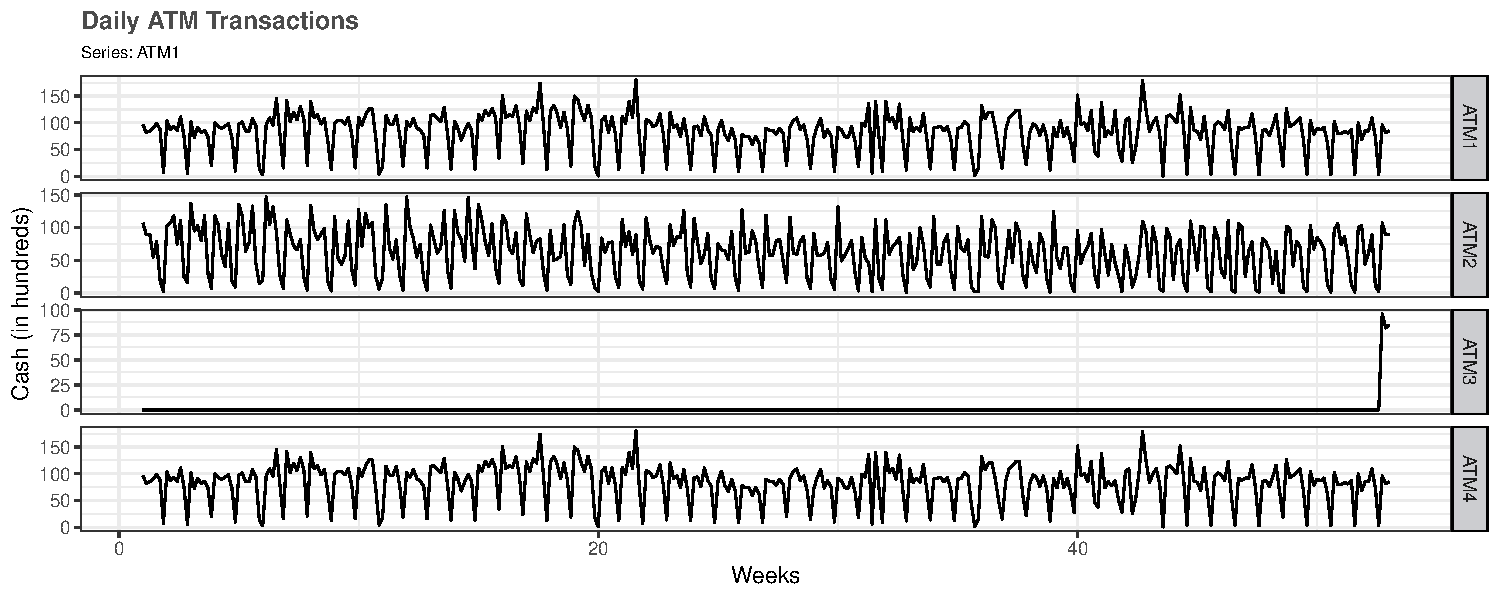
\includegraphics{Part-A-JM_JO_files/figure-latex/unnamed-chunk-4-1.pdf}

\hypertarget{evaluation}{%
\section{Evaluation}\label{evaluation}}

We constructed our initial timeseries for ATM1, ATM2, and ATM4 using a
weekly frequency. Our ACF plots for each ATM showcases large, decreasing
lags starting at 7. This pattern continues in a multiple of seven, which
confirms our assumption about seasonality within the observed data.
These lags are indicative of a weekly pattern. \newline

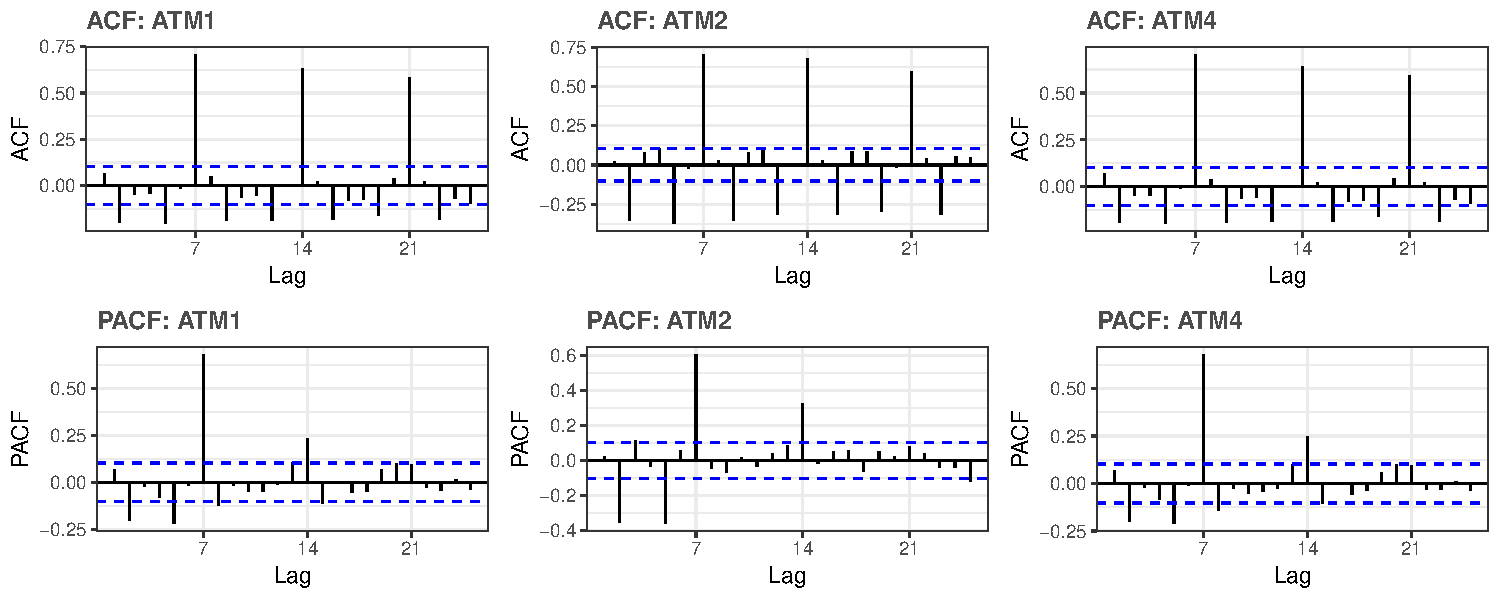
\includegraphics{Part-A-JM_JO_files/figure-latex/unnamed-chunk-5-1.pdf}

Our plots further suggest that the ATM data is non-stationary. We
performed a unit root test using the \texttt{ur.kpss()} function to
confirm this observation. The test results below show that differencing
is required on all ATM2 and ATM4 series. ATM1 falls just below the
cut-off critical value, but could still benefit from differencing due to
the observed seasonal pattern.

\begin{table}[H]

\caption{\label{tab:unnamed-chunk-6}KPSS unit root test}
\centering
\begin{tabular}{l|l|l}
\hline
\textbf{ATM} & \textbf{No-Diff} & \textbf{Diff-1}\\
\hline
\rowcolor{gray!6}  ATM1 & 0.4967 & 0.0219\\
\hline
ATM2 & 2.0006 & 0.016\\
\hline
\rowcolor{gray!6}  ATM4 & 0.5182 & 0.0211\\
\hline
\end{tabular}
\end{table}

\hypertarget{modeling}{%
\subsection{Modeling}\label{modeling}}

We used \texttt{auto.arima()} and set \texttt{D=1} to account for
seasonal differencing of our data to select the best ARIMA models for
ATM1, ATM2, and ATM4. The full models and accuracy statistics for each
series can be viewed in the appendix.

\begin{itemize}
\tightlist
\item
  \textbf{ATM1}: ARIMA\((0,0,2)(0,1,1)_7\)
\item
  \textbf{ATM2}: ARIMA\((2,0,2)(0,1,1)_7\)
\item
  \textbf{ATM3}: MEAN
\item
  \textbf{ATM4}: ARIMA\((0,0,2)(0,1,1)_7\)
\end{itemize}

The residual ACF plots contain no pattern and the lags fall within the
critical value, which suggest they are white noise and not
autocorrelated. Further, the residual histograms follow a relatively
normal distribution, which confirms that the models adequately fits the
observed data.

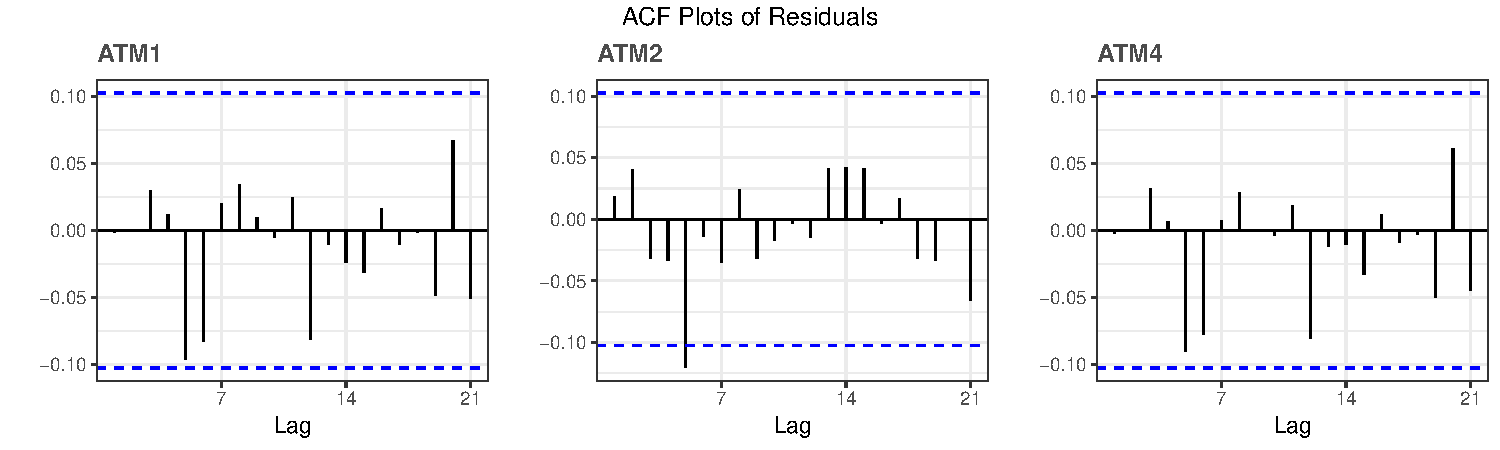
\includegraphics{Part-A-JM_JO_files/figure-latex/unnamed-chunk-7-1.pdf}
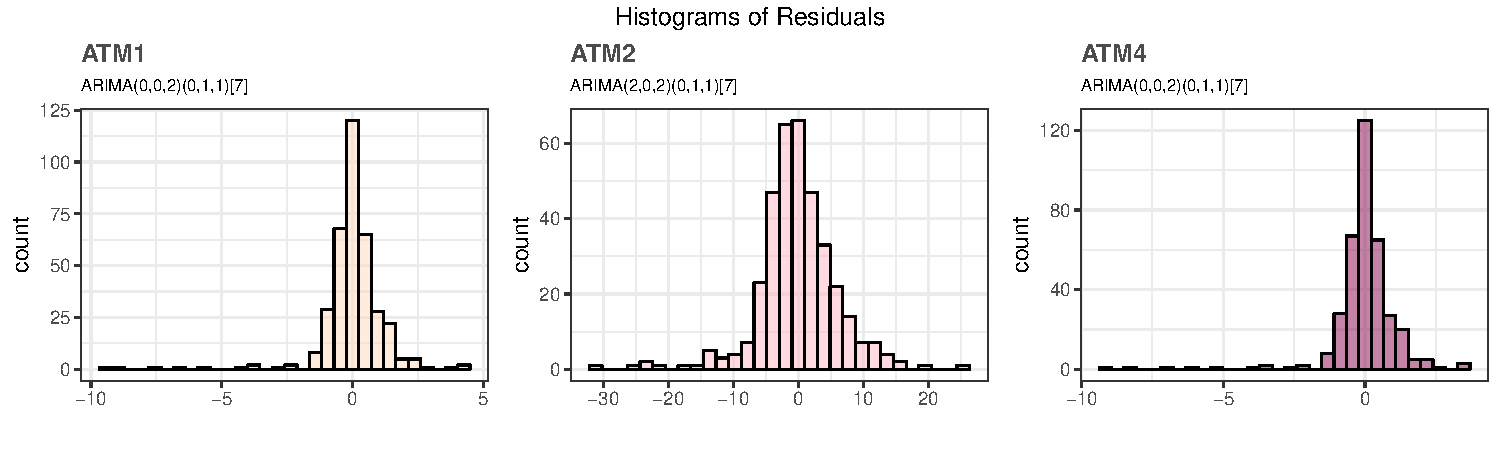
\includegraphics{Part-A-JM_JO_files/figure-latex/unnamed-chunk-7-2.pdf}

\hypertarget{forecast}{%
\section{Forecast}\label{forecast}}

A forecast for the month of May will be 31 days in length. We applied a
forecast to each series for 31 days, which span across 5 weeks, in May
2010. The numeric forecasts can be viewed in a table output in the
appendix section and are also located within our data output folder.

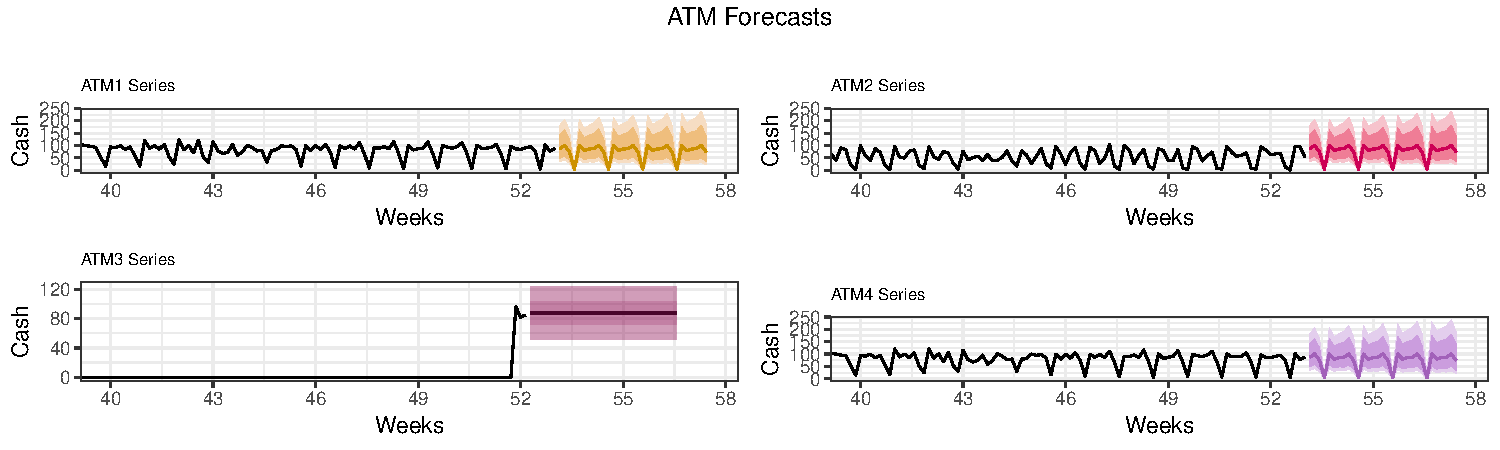
\includegraphics{Part-A-JM_JO_files/figure-latex/unnamed-chunk-8-1.pdf}

\hypertarget{Appendix}{%
\chapter*{Appendix}\label{Appendix}}
\addcontentsline{toc}{chapter}{Appendix}

\hypertarget{Part-A}{%
\section*{Part A}\label{Part-A}}
\addcontentsline{toc}{section}{Part A}

\hypertarget{Part-A-arima}{%
\subsection*{ARIMA Model Summary}\label{Part-A-arima}}
\addcontentsline{toc}{subsection}{ARIMA Model Summary}

\textbf{\texttt{ATM1}:}

\begin{verbatim}
FALSE Series: ATM1_ts 
FALSE ARIMA(0,0,2)(0,1,1)[7] 
FALSE Box Cox transformation: lambda= 0.2584338 
FALSE 
FALSE Coefficients:
FALSE          ma1      ma2     sma1
FALSE       0.1085  -0.1089  -0.6425
FALSE s.e.  0.0524   0.0521   0.0431
FALSE 
FALSE sigma^2 estimated as 1.726:  log likelihood=-606.1
FALSE AIC=1220.2   AICc=1220.32   BIC=1235.72
\end{verbatim}

\textbf{\texttt{ATM2}:}

\begin{verbatim}
FALSE Series: ATM2_ts 
FALSE ARIMA(2,0,2)(0,1,1)[7] 
FALSE Box Cox transformation: lambda= 0.661752 
FALSE 
FALSE Coefficients:
FALSE           ar1      ar2     ma1     ma2     sma1
FALSE       -0.4238  -0.8978  0.4766  0.7875  -0.7064
FALSE s.e.   0.0592   0.0473  0.0883  0.0608   0.0417
FALSE 
FALSE sigma^2 estimated as 38.94:  log likelihood=-1162.96
FALSE AIC=2337.93   AICc=2338.17   BIC=2361.21
\end{verbatim}

\textbf{\texttt{ATM3}:}

\begin{verbatim}
FALSE Mean of non-zero values is 87.67
\end{verbatim}

\textbf{\texttt{ATM4}:}

\begin{verbatim}
FALSE Series: ATM4_ts 
FALSE ARIMA(0,0,2)(0,1,1)[7] 
FALSE Box Cox transformation: lambda= 0.2328582 
FALSE 
FALSE Coefficients:
FALSE          ma1      ma2     sma1
FALSE       0.1095  -0.1088  -0.6474
FALSE s.e.  0.0524   0.0523   0.0420
FALSE 
FALSE sigma^2 estimated as 1.439:  log likelihood=-573.5
FALSE AIC=1154.99   AICc=1155.11   BIC=1170.52
\end{verbatim}

\hypertarget{Part-A-FC}{%
\subsection*{Point Forecasts}\label{Part-A-FC}}
\addcontentsline{toc}{subsection}{Point Forecasts}

\begin{table}[H]

\caption{\label{tab:unnamed-chunk-13}ATM Mean Point Forecast}
\centering
\begin{tabular}{l|l|l|l|l}
\hline
\textbf{Date} & \textbf{ATM1} & \textbf{ATM2} & \textbf{ATM3} & \textbf{ATM4}\\
\hline
\rowcolor{gray!6}  2010-05-01 & 86.6822230334281 & 65.9130078295388 & 87.6666666666667 & 86.7148793513953\\
\hline
2010-05-02 & 100.569237833094 & 71.2678744758685 & 87.6666666666667 & 100.581688969852\\
\hline
\rowcolor{gray!6}  2010-05-03 & 73.710292000956 & 11.4694658108709 & 87.6666666666667 & 73.645362194735\\
\hline
2010-05-04 & 4.22902938718943 & 2.46415237936744 & 87.6666666666667 & 4.22143290375228\\
\hline
\rowcolor{gray!6}  2010-05-05 & 100.159253208527 & 98.3397063045857 & 87.6666666666667 & 100.159422079885\\
\hline
2010-05-06 & 79.3467329167084 & 89.0607216505235 & 87.6666666666667 & 79.3417211032809\\
\hline
\rowcolor{gray!6}  2010-05-07 & 85.7390398914344 & 66.0684601266365 & 87.6666666666667 & 85.7781984478913\\
\hline
2010-05-08 & 87.1797624007239 & 65.9067170158147 & 87.6666666666667 & 87.218337497544\\
\hline
\rowcolor{gray!6}  2010-05-09 & 100.388112929695 & 71.3008782172556 & 87.6666666666667 & 100.395109536387\\
\hline
2010-05-10 & 73.710292000956 & 11.4650527078295 & 87.6666666666667 & 73.645362194735\\
\hline
\rowcolor{gray!6}  2010-05-11 & 4.22902938718943 & 2.45577466621943 & 87.6666666666667 & 4.22143290375228\\
\hline
2010-05-12 & 100.159253208527 & 98.3602657501897 & 87.6666666666667 & 100.159422079885\\
\hline
\rowcolor{gray!6}  2010-05-13 & 79.3467329167084 & 89.0776223553505 & 87.6666666666667 & 79.3417211032809\\
\hline
2010-05-14 & 85.7390398914344 & 66.0458523021009 & 87.6666666666667 & 85.7781984478913\\
\hline
\rowcolor{gray!6}  2010-05-15 & 87.1797624007239 & 65.9025868757576 & 87.6666666666667 & 87.218337497544\\
\hline
2010-05-16 & 100.388112929695 & 71.3235063276986 & 87.6666666666667 & 100.395109536387\\
\hline
\rowcolor{gray!6}  2010-05-17 & 73.710292000956 & 11.4619371370152 & 87.6666666666667 & 73.645362194735\\
\hline
2010-05-18 & 4.22902938718943 & 2.45005983249313 & 87.6666666666667 & 4.22143290375228\\
\hline
\rowcolor{gray!6}  2010-05-19 & 100.159253208527 & 98.3744953596224 & 87.6666666666667 & 100.159422079885\\
\hline
2010-05-20 & 79.3467329167084 & 89.0890848253535 & 87.6666666666667 & 79.3417211032809\\
\hline
\rowcolor{gray!6}  2010-05-21 & 85.7390398914344 & 66.0302973545638 & 87.6666666666667 & 85.7781984478913\\
\hline
2010-05-22 & 87.1797624007239 & 65.8998808213307 & 87.6666666666667 & 87.218337497544\\
\hline
\rowcolor{gray!6}  2010-05-23 & 100.388112929695 & 71.3390190248587 & 87.6666666666667 & 100.395109536387\\
\hline
2010-05-24 & 73.710292000956 & 11.4597394828691 & 87.6666666666667 & 73.645362194735\\
\hline
\rowcolor{gray!6}  2010-05-25 & 4.22902938718943 & 2.44616060460193 & 87.6666666666667 & 4.22143290375228\\
\hline
2010-05-26 & 100.159253208527 & 98.3843423320737 & 87.6666666666667 & 100.159422079885\\
\hline
\rowcolor{gray!6}  2010-05-27 & 79.3467329167084 & 89.0968573387821 & 87.6666666666667 & 79.3417211032809\\
\hline
2010-05-28 & 85.7390398914344 & 66.0195955091203 & 87.6666666666667 & 85.7781984478913\\
\hline
\rowcolor{gray!6}  2010-05-29 & 87.1797624007239 & 65.8981117895746 & 87.6666666666667 & 87.218337497544\\
\hline
2010-05-30 & 100.388112929695 & 71.3496527614802 & 87.6666666666667 & 100.395109536387\\
\hline
\rowcolor{gray!6}  2010-05-31 & 73.710292000956 & 11.4581905724258 & 87.6666666666667 & 73.645362194735\\
\hline
\end{tabular}
\end{table}

\newpage

\hypertarget{Part-A-RScript}{%
\subsection*{R Script}\label{Part-A-RScript}}
\addcontentsline{toc}{subsection}{R Script}

\begin{Shaded}
\begin{Highlighting}[]
\CommentTok{# Dependencies}
\CommentTok{## processing}
\KeywordTok{library}\NormalTok{(readxl)}
\KeywordTok{library}\NormalTok{(tidyverse)}
\KeywordTok{library}\NormalTok{(janitor)}

\CommentTok{## forecasting packages}
\KeywordTok{library}\NormalTok{(urca)}
\KeywordTok{library}\NormalTok{(forecast)}
\KeywordTok{library}\NormalTok{(fpp2)}

\CommentTok{# Load data}
\NormalTok{atm_data <-}\StringTok{ }\KeywordTok{read_excel}\NormalTok{(}\StringTok{"data/ATM624Data.xlsx"}\NormalTok{) }

\CommentTok{# clean dataframe}
\NormalTok{atm <-}\StringTok{ }\NormalTok{atm_data }\OperatorTok\StringTok{ }
\StringTok{  }\CommentTok{# create wide dataframe}
\StringTok{  }\KeywordTok{spread}\NormalTok{(ATM, Cash) }\OperatorTok\StringTok{ }
\StringTok{  }\CommentTok{# remove NA column using function from janitor package}
\StringTok{  }\KeywordTok{remove_empty}\NormalTok{(}\DataTypeTok{which =} \StringTok{"cols"}\NormalTok{) }\OperatorTok
\StringTok{  }\CommentTok{# filter unobserved values from May 2010}
\StringTok{  }\KeywordTok{filter}\NormalTok{(DATE }\OperatorTok{<}\StringTok{ }\KeywordTok{as.Date}\NormalTok{(}\StringTok{"2010-05-01"}\NormalTok{)) }\OperatorTok
\StringTok{  }\CommentTok{# ensure dates are ascending}
\StringTok{  }\KeywordTok{arrange}\NormalTok{(DATE) }

\NormalTok{atm}\OperatorTok{$}\NormalTok{ATM2[}\KeywordTok{is.na}\NormalTok{(atm}\OperatorTok{$}\NormalTok{ATM2)] <-}\StringTok{ }\KeywordTok{mean}\NormalTok{(atm}\OperatorTok{$}\NormalTok{ATM2, }\DataTypeTok{na.rm =} \OtherTok{TRUE}\NormalTok{) }\CommentTok{## remove NA}
\NormalTok{atm}\OperatorTok{$}\NormalTok{ATM4[}\KeywordTok{which.max}\NormalTok{(atm}\OperatorTok{$}\NormalTok{ATM4)] <-}\StringTok{ }\KeywordTok{mean}\NormalTok{(atm}\OperatorTok{$}\NormalTok{ATM4, }\DataTypeTok{na.rm =} \OtherTok{TRUE}\NormalTok{) }\CommentTok{## remove outlier}

\CommentTok{# create TS with weekly frequency & subset data}
\NormalTok{atm_ts <-}\StringTok{ }\NormalTok{atm }\OperatorTok\StringTok{ }\KeywordTok{select}\NormalTok{(}\OperatorTok{-}\NormalTok{DATE) }\OperatorTok\StringTok{ }\KeywordTok{ts}\NormalTok{(}\DataTypeTok{start=}\DecValTok{1}\NormalTok{,  }\DataTypeTok{frequency =} \DecValTok{7}\NormalTok{)}
\NormalTok{ATM1_ts <-}\StringTok{ }\NormalTok{atm_ts[,}\DecValTok{1}\NormalTok{]; ATM2_ts <-}\StringTok{ }\NormalTok{atm_ts[,}\DecValTok{2}\NormalTok{]; ATM3_ts <-}\StringTok{ }\NormalTok{atm_ts[,}\DecValTok{3}\NormalTok{]; ATM4_ts <-}\StringTok{ }\NormalTok{atm_ts[,}\DecValTok{4}\NormalTok{]}

\CommentTok{#unit root test}
\CommentTok{## no diff}
\NormalTok{ATM1_ur <-}\KeywordTok{ur.kpss}\NormalTok{(ATM1_ts)}
\NormalTok{ATM2_ur <-}\KeywordTok{ur.kpss}\NormalTok{(ATM2_ts)}
\NormalTok{ATM4_ur <-}\KeywordTok{ur.kpss}\NormalTok{(ATM4_ts)}
\CommentTok{## first order diff}
\NormalTok{ATM1d_ur <-}\KeywordTok{ur.kpss}\NormalTok{(}\KeywordTok{diff}\NormalTok{(ATM1_ts, }\DataTypeTok{lag=}\DecValTok{7}\NormalTok{))}
\NormalTok{ATM2d_ur <-}\KeywordTok{ur.kpss}\NormalTok{(}\KeywordTok{diff}\NormalTok{(ATM2_ts, }\DataTypeTok{lag=}\DecValTok{7}\NormalTok{))}
\NormalTok{ATM4d_ur <-}\KeywordTok{ur.kpss}\NormalTok{(}\KeywordTok{diff}\NormalTok{(ATM4_ts, }\DataTypeTok{lag=}\DecValTok{7}\NormalTok{))}

\CommentTok{# AUTO.ARIMA function; set D=1 for seasonal differencing}
\NormalTok{ATM1_AA <-}\KeywordTok{auto.arima}\NormalTok{(ATM1_ts, }\DataTypeTok{D =} \DecValTok{1}\NormalTok{, }\DataTypeTok{lambda =} \StringTok{"auto"}\NormalTok{, }\DataTypeTok{approximation =}\NormalTok{ F, }\DataTypeTok{stepwise =}\NormalTok{ T)}
\NormalTok{ATM2_AA <-}\KeywordTok{auto.arima}\NormalTok{(ATM2_ts, }\DataTypeTok{D =} \DecValTok{1}\NormalTok{, }\DataTypeTok{lambda =} \StringTok{"auto"}\NormalTok{, }\DataTypeTok{approximation =}\NormalTok{ F, }\DataTypeTok{stepwise =}\NormalTok{ T)}
\NormalTok{ATM4_AA <-}\KeywordTok{auto.arima}\NormalTok{(ATM4_ts, }\DataTypeTok{D =} \DecValTok{1}\NormalTok{, }\DataTypeTok{lambda =} \StringTok{"auto"}\NormalTok{, }\DataTypeTok{approximation =}\NormalTok{ F, }\DataTypeTok{stepwise =}\NormalTok{ T)}

\CommentTok{# Forecast Results}
\NormalTok{ATM1_fc <-}\StringTok{ }\KeywordTok{forecast}\NormalTok{(ATM1_AA,}\DataTypeTok{h=}\DecValTok{31}\NormalTok{)}
\NormalTok{ATM2_fc <-}\StringTok{ }\KeywordTok{forecast}\NormalTok{(ATM2_AA,}\DataTypeTok{h=}\DecValTok{31}\NormalTok{)}
\NormalTok{ATM3_fc <-}\StringTok{ }\KeywordTok{meanf}\NormalTok{(ATM3_ts[ATM3_ts }\OperatorTok{>}\StringTok{ }\DecValTok{0}\NormalTok{], }\DataTypeTok{h=}\DecValTok{31}\NormalTok{)}\CommentTok{# based on three non-zero values (between observations 363 and 365)}
\NormalTok{ATM4_fc <-}\StringTok{ }\KeywordTok{forecast}\NormalTok{(ATM4_AA,}\DataTypeTok{h=}\DecValTok{31}\NormalTok{)}

\CommentTok{# Prepare dataframe for ATM3 mean forcast plotting }
\NormalTok{ATM3_plotdata_fc <-}\StringTok{ }\KeywordTok{cbind}\NormalTok{(}\KeywordTok{seq}\NormalTok{(}\DataTypeTok{from =} \DecValTok{366}\NormalTok{, }\DataTypeTok{to =} \DecValTok{396}\NormalTok{),}
\NormalTok{                          ATM3_fc[[}\DecValTok{5}\NormalTok{]], }
\NormalTok{                          ATM3_fc[[}\DecValTok{6}\NormalTok{]], }
\NormalTok{                          ATM3_fc[[}\DecValTok{7}\NormalTok{]]) }\OperatorTok\StringTok{ }
\StringTok{  }\KeywordTok{as.data.frame}\NormalTok{()}

\KeywordTok{colnames}\NormalTok{(ATM3_plotdata_fc) <-}\StringTok{ }\KeywordTok{c}\NormalTok{(}\StringTok{'Date'}\NormalTok{, }\StringTok{'Point Forecast'}\NormalTok{, }\StringTok{'Lo 80'}\NormalTok{, }\StringTok{'Lo 95'}\NormalTok{, }\StringTok{'Hi 80'}\NormalTok{, }\StringTok{'Hi 95'}\NormalTok{)}
\NormalTok{ATM3_plotdata <-}\StringTok{ }\NormalTok{ATM3_ts }\OperatorTok\StringTok{ }
\StringTok{  }\KeywordTok{fortify}\NormalTok{() }\OperatorTok\StringTok{ }
\StringTok{  }\KeywordTok{select}\NormalTok{(}\OperatorTok{-}\NormalTok{Index) }\OperatorTok
\StringTok{  }\KeywordTok{rename}\NormalTok{(}\DataTypeTok{Cash =}\NormalTok{ Data) }\OperatorTok\StringTok{ }
\StringTok{  }\KeywordTok{mutate}\NormalTok{(}\DataTypeTok{Date =} \KeywordTok{as.numeric}\NormalTok{(}\KeywordTok{row.names}\NormalTok{(.))) }\OperatorTok\StringTok{ }
\StringTok{  }\KeywordTok{select}\NormalTok{(Date, Cash) }\OperatorTok\StringTok{ }
\StringTok{  }\KeywordTok{full_join}\NormalTok{(ATM3_plotdata_fc, }\DataTypeTok{by =} \StringTok{'Date'}\NormalTok{)}

\CommentTok{#Revert results back into original form}
\NormalTok{date <-}\StringTok{ }\KeywordTok{as.character}\NormalTok{(}\KeywordTok{seq}\NormalTok{(}\KeywordTok{as.Date}\NormalTok{(}\StringTok{'2010-05-01'}\NormalTok{), }\DataTypeTok{length.out=}\DecValTok{31}\NormalTok{, }\DataTypeTok{by=}\DecValTok{1}\NormalTok{))}
\NormalTok{ATM_FC <-}\StringTok{  }\KeywordTok{cbind}\NormalTok{(}\StringTok{"Date"}\NormalTok{=date, }
                 \StringTok{"ATM1"}\NormalTok{=ATM1_fc}\OperatorTok{$}\NormalTok{mean, }
                 \StringTok{"ATM2"}\NormalTok{=ATM2_fc}\OperatorTok{$}\NormalTok{mean,}
                 \StringTok{"ATM3"}\NormalTok{=ATM3_fc}\OperatorTok{$}\NormalTok{mean,}
                 \StringTok{"ATM4"}\NormalTok{=ATM4_fc}\OperatorTok{$}\NormalTok{mean) }\OperatorTok\StringTok{ }\KeywordTok{as.data.frame}\NormalTok{()}

\KeywordTok{write_csv}\NormalTok{(ATM_FC, }\DataTypeTok{path =} \StringTok{"forecasts/ATM_all_forecast.csv"}\NormalTok{)}
\end{Highlighting}
\end{Shaded}


\end{document}
